% def.tex

% File containing LaTeX macros.
% Has grown by accretion; can be better organized.

\documentclass{article}
\usepackage{amsmath}
\usepackage{amssymb}
\usepackage{bm}
\usepackage{graphicx}
\usepackage{epstopdf}
\DeclareGraphicsRule{.tif}{png}{.png}{`convert #1 `basename #1 .tif`.png}
\usepackage{color}
\usepackage{pdfsync}
\pagestyle{plain}

%\pagestyle{empty}

\textheight 9 true in
\textwidth 6.5 true in
\hoffset -.75 true in
\voffset -.75 true in
 \mathsurround=2pt  \parskip=2pt
\def\crv{\cr\noalign{\vskip7pt}} 

\def\a{\alpha } \def\b{\beta } \def\d{\delta } \def\D{\Delta } \def\e{\epsilon }
\def\g{\gamma } \def\G{\Gamma} \def\k{\kappa} \def\l{\lambda } \def\L{\Lambda }
\def\th{\theta } \def\Th{\Theta} \def\r{\rho} \def\o{\omega} \def\O{\Omega}
\def\ve{\varepsilon} 

\def\sA{{\cal A}} \def\sB{{\cal B}} \def\sC{{\cal C}} \def\sE{{\cal E}} \def\sI{{\cal I}}
\def\sR{{\cal R}} \def\sF{{\cal F}} \def\sG{{\cal G}} \def\sM{{\cal M}}
\def\sT{{\cal T}} \def\sH{{\cal H}} \def\sD{{\cal D}} \def\sW{{\cal W}}
\def\sL{{\cal L}} \def\sP{{\cal P}} \def\s{\sigma } \def\S{\Sigma}
\def\sU{{\cal U}} \def\sY{{\cal Y}}

\def\gm{\gamma -1}
\def\summ{\sum_{j=1}^4}

\def\bb{{\bm b}} \def\yb{{\bm y}}
\def\ub{{\bm u}}  \def\xb{{\bm x}} \def\vb{{\bm v}} \def\wb{{\bm w}}
\def\omegab{{\bm \omega}} \def\rb{{\bm r}} \def\ib{{\bm i}} \def\jb{{\bm j}}
\def\lb{{\bm l}} \def\kb{{\bm k}} \def\Ab{{\bm A}} \def\fb{{\bm f}} \def\Ub{{\bm U}}
\def\Fb{{\bm F}} \def\nb{{\bm n}} \def\Db{{\bm D}} \def\eb{{\bm e}}
\def\gb{{\bm g}}  \def\hb{{\bm h}} \def\Yb{{\bm Y}} \def\Rb{{\bm R}} 

\def\As1{{\bf {\cal A}}_1}\def\DO{{\cal D}_0} \def\UO{{\cal U}_0}
\def\ie{{\it{i.e.}}}

\def\ubbar{{\bf {\bar{u}}}} \def\sbar{{\bar{\sigma }}} \def\ubar{{\bar{u}}}  
\def\abar{{\bar{a}}} \def\vbar{{\bar{v}}}  \def\rbar{{\bar{\rho}}}
\def\pbar{{\bar{p}}} \def\ebar{{\bar{e}}} \def\Tbar{{\bar{T}}}
\def\bbar{{\bar{\beta}}} \def\Mbar{{\bar{M}}}  \def \sMbar{{\bar{\cal M}}}
\def\Ebar{{\bar{E}}} \def\sMbar{{\bar{\cal M}}}
\def\sPbar{{\bar{\cal P}}} \def\xbar{{\bar{x}}}

\newcommand{\pdv}[2]{\frac{\partial#1}{\partial#2}}
\newcommand{\dv}[2]{\frac{d#1}{d#2}}
\newcommand{\ord}[2]{#1^{(#2)}}
\newcommand{\vct}[1]{\vec{#1}}

 \newcommand{\bc}{\begin{center}}
 \newcommand{\ec}{\end{center}}
 
 \newcommand{\bq}{\begin{equation}}
 \newcommand{\eq}{\end{equation}}
 
 \newcommand{\beqs}{\begin{eqnarray}}
 \newcommand{\eeqs}{\end{eqnarray}}
 
 \newcommand{\beqa}{\begin{eqnarray*}}
 \newcommand{\eeqa}{\end{eqnarray*}}
 
 \newcommand{\ol}{\overline}
 \newcommand{\ul}{\underline}
 
 \newcommand{\dint}{{\int \!\! \int \!\!}}
 \newcommand{\tint}{{\int \!\! \int \!\! \int \!\!}}
 
 \newcommand{\bfig}{\begin{figure}}
 \newcommand{\efig}{\end{figure}}
 
 \newcommand{\cen}{\centering}
 \newcommand{\n}{\noindent}
 
 \newcommand{\btab}{\begin{table}}
 \newcommand{\etab}{\end{table}}
 
 \newcommand{\btbl}{\begin{tabular}}
 \newcommand{\etbl}{\end{tabular}}
 
 \newcommand{\bdes}{\begin{description}}
 \newcommand{\edes}{\end{description}}
 
 \newcommand{\benum}{\begin{enumerate}}
 \newcommand{\eenum}{\end{enumerate}}
 
 \newcommand{\bite}{\begin{itemize}}
 \newcommand{\eite}{\end{itemize}}
 
 \newcommand{\cle}{\clearpage}
 \newcommand{\npg}{\newpage}
 
 \newcommand{\bss}{\begin{singlespace}}
 \newcommand{\ess}{\end{singlespace}}
 
 \newcommand{\bhalf}{\begin{onehalfspace}}
 \newcommand{\ehalf}{\end{onehalfspace}}
 
 \newcommand{\bds}{\begin{doublespace}}
 \newcommand{\eds}{\end{doublespace}}
 
 \newcommand{\eps}{\mbox{$\epsilon$}} 
 \newcommand{\stilde}{\mbox{$\tilde s$}} 
 \newcommand{\shat}{\mbox{$\hat s$}} 

 \newcommand{\blue}{\color{blue}}
 \newcommand{\red}{\color{red}}
 \newcommand{\magenta}{\color{magenta}}
 \newcommand{\green}{\color{green}}
 \newcommand{\nc}{\normalcolor}



\def\arg{{\rm{arg}}}
\def\Arg{{\rm{Arg}}}
\def\imath{i}
\def\Log{{\rm{Log}}}
\def\erfc{{\rm{erfc}}}
\def\Oh{\mathcal{O}}
\def\oh{\mathsf{o}}

\def\Res{{\rm{Res}}}

\def\fl{{\rm{fl}}}

\def\Xint#1{\mathchoice
{\XXint\displaystyle\textstyle{#1}}%
{\XXint\textstyle\scriptstyle{#1}}%
{\XXint\scriptstyle\scriptscriptstyle{#1}}%
{\XXint\scriptscriptstyle\scriptscriptstyle{#1}}%
\!\int}
\def\XXint#1#2#3{{\setbox0=\hbox{$#1{#2#3}{\int}$ }
\vcenter{\hbox{$#2#3$ }}\kern-.6\wd0}}
\def\ddashint{\Xint=}
\def\dashint{\Xint-}

%\numberwithin{equation}{section}
\pagestyle{empty}
\begin{document}
Wang Xinshi 661975305\\
\begin{center}
\large{ MATH-2400 \hspace{.25in}  INTRODUCTION TO DIFFERENTIAL EQUATIONS \hspace{.25in}SPRING 2021\\ Homework-3   \\ Assigned Friday Feb 12, 2021 \\ Due 12:00 Noon, Friday Feb 19, 2021}\end{center}

\bigskip
\n\ul{NOTES}
\benum
\item 
Practice problems listed below and taken from the textbook are for your own practice, and are not to be turned in.
\item 
Legible, handwritten solutions will be acceptable, but the use of a typesetting system such as LaTeX is strongly recommended.  \blue{\bf Do not turn in your rough attempt at solving a problem; once you have worked out the solution, copy it neatly or typeset it before submission, after removing all false starts.}\nc
\item 
Please write your solutions clearly and coherently, with the work displayed in a sequential manner and sufficient explanation provided so that your strategy and approach are transparent to the reader. 
\item 
Figures, if any, should be neatly drawn by hand, properly labelled and captioned.  
\item 
The assignment is to be submitted electronically to LMS  as a single pdf file.  Be sure that the pages are properly oriented and well lighted.  \blue{\bf Please do not e-mail your homework submission to the TAs or the instructors.}\nc
\eenum

\bigskip


\bc {\bf Practice Problems from the textbook (not to be turned in)} \ec

\n Exercises from Chapter 3, page 44: 2, 4, 5.\\
\n Exercises from Chapter 3, pages 50-51: 3e, 3g, 4c, 4g, 6a, 6b.


\medskip
\bc {\bf Subjective part: problems to be turned in} \ec

\begin{enumerate}



% Problem 1
\item (20 points)  
A pond forms as water collects in a conical depression of radius $R$ and depth $H.$ Suppose that water flows in at a constant rate $k$ (volume/time) and is lost through evaporation at a rate $\a S$ (volume/time) where $S$ is surface area of water in the pond and $\a,$ the coefficient of evaporation, is a constant.

\benum
\item 
At time $t$ let $r(t)$ be the radius of the water surface and $h(t)$ its height.  Write down an expression for $h(t)$ as a function of $r(t).$

As we know, the water in the pond has a similar shape with pond itself. Thus we have $\dfrac{r(t)}{h(t)} = \dfrac{R}{H}$. Thus we know $h(t) = \dfrac{Hr(t)}{R}$.
\item Write down an expression for the volume of water in the pond, $V(t),$ as a function of $r(t).$

\begin{align*}
	V(t) &= \dfrac{1}{3} \pi r(t)^2 h(t)\\
	V(t) & = \dfrac{1}{3} \pi r(t)^2 \dfrac{Hr(t)}{R}\\
	V(t) & = \dfrac{1}{3} \pi \dfrac{Hr^3(t)}{R}\\
\end{align*}

\item Write down an expression for $S(t),$ the area of the exposed water surface.

First we need to express $r(t)$ in terms of constants. We compute $r(t)$ from $V$
\begin{align*}
	V(t) & = \dfrac{1}{3} \pi \dfrac{Hr^3(t)}{R}\\
	3VR &= \pi H r(t)^3\\
	r(t) &= (\dfrac{3VR}{\pi H})^{\dfrac{1}{3}} 
\end{align*}
$$S(t) = \pi r(t)^2 = \pi( \dfrac{3VR}{\pi H})^{\dfrac{2}{3}} $$
\item Show that $V(t)$ satisfies the DE
\begin{equation*}
V'(t) = k - \a \pi \left(\frac{3RV}{\pi H}\right)^{2/3}.
\end{equation*}

We know that $V'(t) = k - \a S(t)$. Substituting the result from (c) we get:
\begin{align*}
	V'(t) &= k - \a S(t).\\
	V'(t) &= k - \a \pi ( \dfrac{3VR}{\pi H})^{\dfrac{2}{3}}.\\
	V'(t) &= k - \a \pi \left(\frac{3RV}{\pi H}\right)^{\dfrac{2}{3}}.
\end{align*} 
\item Find the equilibrium depth of water in the pond and determine if the equilibrium is stable or unstable.

To find the equilibrium depth, we set $\dfrac{dV}{dt} = 0$. Then we have 
\begin{align*}
	 &k - \a \pi \left(\frac{3RV}{\pi H}\right)^{\dfrac{2}{3}} = 0\\
	 &k = \a \pi \left(\frac{3R}{\pi H}\right)^{\dfrac{2}{3}} V^{\dfrac{2}{3}}\\
	 &(\dfrac{k}{\a \pi})^{\dfrac{3}{2}} = \dfrac{3R}{\pi H} V\\
	 &V = \pm \dfrac{(\dfrac{k}{\a \pi})^{\dfrac{3}{2}} \pi H}{3R}
\end{align*}

We discard the negative value for practical reason. 

Substituting $V$ into $r(t) = (\dfrac{3VR}{\pi H})^{\dfrac{1}{3}}$, we have $$r(t) = (\dfrac{(\dfrac{k}{\a \pi})^{\dfrac{3}{2}} \pi H}{\pi H})^{\dfrac{1}{3}}$$
$$r(t) = (\dfrac{k}{\a \pi})^{\dfrac{1}{2}}$$

Thus from the formula we derived in a, $h(t) = \dfrac{H(\dfrac{k}{\a \pi})^{\dfrac{1}{2}}}{R}$.\\
	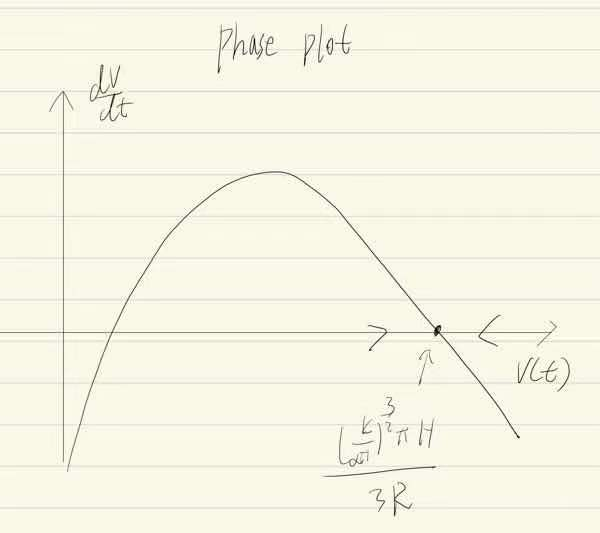
\includegraphics[scale = 0.3]{"C:/Users/Micha/OneDrive - Rensselaer Polytechnic Institute/MATH2400/pictures/stable.jpg"}\\
From the phase plot we draw, we know it is stable equilibrium.\\\\
\item What condition must the flow rate $k$ satisfy if the pond is not to overflow?
\eenum

Intuitively, the pond will not overflow if its equilibrium volumn is equal to the designated value. $\dfrac{1}{3} \pi H R^2 = \dfrac{(\dfrac{k}{\a \pi})^{\dfrac{3}{2}} \pi H}{3R}$. We then have 
\begin{align*}
	\dfrac{1}{3} R^3 = \dfrac{(\dfrac{k}{\a \pi})^{\dfrac{3}{2}}}{3}\\
	R^3 = (\dfrac{k}{\a \pi})^{\dfrac{3}{2}}\\
	R^2 = \dfrac{k}{\a \pi}\\
	k = R^2 \a \pi
\end{align*}
\newpage

% Problem 2
\item (20 points)  
Solve the following initial-value problems.
\benum
\item $y''-y'-6y=0, \quad y(0)=5, \; y'(0)=0.$\\
Let $y = e^{rt}$, then we have $$y'' = r^2e^{rt}$$ $$y' = re^{rt}$$  $$y = e^{rt}$$

Substitute those values into the original DE gives us the characteristic equation: $$(r^2-r-6)e^{rt} = 0$$

We can factor the equation into $(r-3)(r+2) = 0$, which gives us $r = 3$ and $r = -2$. Therefore we have $y_1(t) = e^{3t}$ and $y_2(t) = e^{-2t}$. Combining those two gives us $$y(t) = C_1e^{3t}+C_2e^{-2t}$$

After taking the derivative, we have $$y'(t) = 3C_1e^{3t}-2C_2e^{-2t}$$

Substituting the IC in, we have 
\begin{equation*}
	\begin{cases}
		C_1+C_2 &= 5\\
		3C_1 - 2C_2 &= 0
	\end{cases}
\end{equation*}

Thus we have $C_1 = 2$ and $C_2 = 3$. Thus the solution is $y(t) = 2e^{3t}+3e^{2t}$.
\item $4y''-12y'+9y=0, \quad y(0)=4, \; y'(0)=5.$
Let $y = e^{rt}$, then we have $$y'' = r^2e^{rt}$$ $$y' = re^{rt}$$  $$y = e^{rt}$$

Substitute those values into the original DE gives us the characteristic equation: $$(4r^2-12r+9)e^{rt} = 0$$

We can factor the equation into $(2r-3)^2= 0$, which gives us $r = \dfrac{3}{2}$. Therefore we the general solution directly from the \textbf{Remark} section in lecture 06: $$y(t) = C_1e^{\dfrac{3}{2}t}+C_2te^{\dfrac{3}{2}t}$$  
After taking the derivative, we have $$y'(t) = \dfrac{3}{2}C_1e^{\dfrac{3}{2}t}+C_2e^{\dfrac{3}{2}t}\dfrac{3}{2}+C_2te^{\dfrac{3}{2}}$$


Substituting the IC in, we have 
\begin{equation*}
	\begin{cases}
		C_1 &= 4\\
		\dfrac{3}{2}C_1 + C_2 &= 5
	\end{cases}
\end{equation*}

Thus we have $C_1 = 4$ and $C_2 = -1$. Thus the solution is $y(t) = 4e^{\dfrac{3}{2}t}-te^{\dfrac{3}{2}t}$.
\eenum

\newpage

% Problem 3
\item (20 points)
Consider the DE
\begin{equation*}
ty''-(t+2)y'+2y=0.
\end{equation*}
\benum
\item Check that $y=e^t$ is a solution of the DE.
 
We know $$y'' = y' = y = e^t$$. We then need to check if the LHS equal to the RHS.\\
LHS: $te^{t}-(t+2)e^{t}+2e^{t}=te^{t}-te^{t}-2e^{t}+2e^{t}=0$\\
RHS: $0$\\
Since the LHS matches the RHS, $y=e^t$ is a valid solution.

\item Use the method of reduction of order to find the general solution of the DE.
\eenum

\hspace*{0.8cm} Let $y_1 = e^{rt}$, then we have $y_2 = w(t)e^{rt}$. Then we have $$y_2'(t) = w'(t)e^t$$  $$y_2''(t) = w''(t) e^t + w'(t)e^t + w'(t)e^t + w(t)e^t$$

Substituting the $y'(t)$ and $y''(t)$ into the differential equation gives us 
\begin{align*}
	(tw''+2tw +tw - (t+2)(w'+w)+2w)e^t = 0 \\
	(tw'' + 2tw' +tw -tw' - 2w' - tw -2w +2w)e^t = 0\\
	(tw''+ tw' -2w')e^rt = 0
\end{align*}
Thus we know $w(t)''+(1-\dfrac{2}{t})w' = 0 $. We replace $w'$ with $u$. Then we have $tu'+(1-\dfrac{2}{t})u = 0$. We can use integrating factor to solve this problem. Let $\mu(t) = e^{\int (1-\dfrac{2}{t})dt} = e^{t-lnt^2} = \dfrac{e^t}{t^2}$. Then we have 
\begin{align*}
	\dfrac{du}{dt}(\dfrac{e^t}{t^2}u) = 0\\
	u = \dfrac{t^2C}{e^t}
\end{align*}
Therefore $w = \int u(t)dt = C \int \dfrac{t^2}{e^t} dt$. We let $f = t^2, dg = e^{-t}dt, f = t^2,$ and $g = -e^{-t}$. Then we have $w = -e^{-t}t^2+2 \int e^{-t} tdt$. Then we let $f = t, dg = e^{-t}dt, df = dt,$ and $g = -e^{-t}$. We have $w = -2e^{-t}-e^{-t}t^2+2\int e^{-t} dt = -(t^2-2t-2)e^{-t}$. Thus $y_2 = wy_1 =  -(t^2-2t-2)e^{-t} \times e^{t} = -(t^2-2t-2)$.\\\\
Therefore $y = C_1e^t+C_2(-t^2+2t+2)$
\end{enumerate}



\end{document}